%!TEX root = ../main.tex

\chapter[The Structure and Evolution of Story Networks]{The Structure and Evolution of Story Networks}\label{ch:story-networks}

\chapterprecishere{``I, too, feel the need to reread the books I have already read,'' a third reader says, ``but at every rereading I seem to be reading a new book, for the first time. Is it I who keep changing and seeing new things of which I was not previously aware? Or is reading a construction that assumes form, assembling a great number of variables, and therefore something that cannot be repeated twice according to the same pattern?''}{Italo Calvino}{If on a Winter's Night a Traveler}

\section{Introduction}\label{sec:networks-introduction}

In his thought-provoking study \emph{Fairy Tale in the Ancient World}, Graham Anderson quotes the following passage by the Greek geographer Strabo (first century BC/AD), which tells the story of a girl called Rhodopis:
\begin{quote}
  ``They tell the fabulous story (\emph{mytheuousi}) that while she was bathing, an eagle seized one of her shoes from her maid and brought it to Memphis, and while the king was dispensing justice in the open air, the eagle arrived over his head and threw the shoe into his lap. The king was aroused by the \emph{rythmos} of the sandal and the strangeness of the event, and sent all around the country in search of the woman who wore it. When she was found in Naucratis she was brought up country to Memphis and became the king's wife.''~\autocite{Anderson:2000}
\end{quote}
Does this sound familiar? The `seizure of the girl's shoe', the `slipper test' and the `marriage to the prince' are all motifs that resonate one of the best known fairy tales in modern times: \emph{Cinderella}.\footnote{In fact, Rhodopis' story exhibits three of the five main characteristics attributed to the Cinderella story type (as characterized by Aarne \& Thompson~\autocite{aarne:1961} in the folktale catalog \emph{The Types of the Folktale}): help of an animal (2), proof of identity (4) and marriage with the prince (5).} The `Cinderella' story as we know it today is derived from Charles Perrault's story \emph{Cendrillon} (from \emph{Contes du temps passé avec moralités}, 1697). Perrault's retelling adds various elements to the story, of which the following two are mentioned in the folktale catalog by Aarne \& Thompson: a persecuted heroine (1) and a meeting with the prince in advance of the slipper test (3)~\autocite{aarne:1961}. Ever since Perrault published his version of the story, \emph{Cinderella}\/ has been retold to new audiences through a variety of channels: books, picture books, films, advertisements, comics, cartoons, and so forth. Yet, these retellings of \emph{Cinderella}\/ do not necessarily derive from Perrault's version. In fact, as Stephens \& McCallum state, it is more likely that retellers ``use intermediate versions -- to produce a retelling of a retelling''\autocite{stephens_mccallum}. These `retellings of retellings', I wish to argue, can be considered as the implicit formation of a network of stories, in which links between stories represent pre-textual relationships\autocite[In evolutionary terms, such networks can be described as lineages or phylogenetic trees. I prefer to use the term network, however, because it does not presume a clear `root node' from which all subsequent story versions have supposedly sprang. Cf.][]{mesoudi:2011, tehrani:2013}. A story network represents a stream of retellings in which retellers modify and adapt retellings in a gradual and accumulative way.

The aim of this chapter is to offer new perspectives on the structure and development of such story networks. More specifically, I am interested in the dynamics and mechanisms that underly retellers' choices for particular story versions to base their retellings on. Certain retellings seem to be more attractive than others, making them more likely candidates for further retelling. Arguably, attractiveness can be defined in two ways: \emph{content-based} and \emph{context-based} attractiveness.\autocite[These types resemble the concepts of content-based and context-based biases in theoretical models of cultural evolution. Cf.][]{henrich:2003} \emph{Content-based attractiveness} concerns inherent aspects of a story which increase or decrease its likelihood of being retold. For instance, Charles Perrault's retelling of ``Little Red Riding Hood'' was highly popular until the Brothers Grimm published their version of ``Rothkäpchen'' in the \nth{19} century. Zipes' thesis is that the Brothers Grimm ``virtually dwarfed Perrault's version'' by the end of the \nth{19} century, because their emphasis on obedience and good behavior was a better fit for the emerging Victorian image of the child\autocite{zipes:1993}. With \emph{context-based} attractiveness, on the other hand, dispositions for certain stories are not determined by inherent features, but, for example, by social factors, such as popularity or prestige of a particular author. Both content-based and context-based attractiveness have received a wealth of attention in literary and folkloristic studies of story transmission\autocite{geerts:2014}. However, despite being suggestive and thought-provoking, informal verbal arguments such as Zipes' account of ``Red Riding Hood'', cannot generate specific predictions which can be quantitatively tested and systematically compared to real-world data. 

A more parsimonious explanation for the preference of a reteller for particular story versions is that there are no real `motivations' or selection criteria underlying their choices, or, in other words, that their choice is completely random. A large number of studies in evolutionary anthropology and cultural evolution has shown that social transmission can often be characterized as an \emph{unbiased} process in a neutral model of selection in which changes are reduced to `random' frequency effects of competing cultural traits~\autocite{Bentley:2004,Mesoudi:2009,bentley:2011}. In the case of story transmission, this would mean that stories with high circulation numbers are more readily available and, in the absence of content- and context-based biases, their attractiveness would be entirely proportional to these numbers. However, if we take enticing accounts of story transmission such as the one by Zipes seriously, it seems unlikely that the selection of a particular story for retelling is entirely frequency-based.

In this study, I wish to depart from the hypothesis that a story's attractiveness for further retelling is merely a `random' frequency effect -- or, in other words, is driven by \emph{frequency-based attractiveness} -- by systematically investigating the possible influence of other attractiveness factors. First, besides \emph{frequency-based attractiveness}, stories might be differentially preferred given their \emph{temporal attractiveness}, which is a form of context-based attractiveness. For instance, it has been shown for academic citation networks that relatively young research is preferred over older studies and that the probability of being cited decays with time~\autocite{dorogovtsev:2000,eom:2011,price:1976,Perc:2014}. Following Stephens \& McCallum, I investigate whether this process equally applies to story networks and whether retellers prefer more recent story versions over older ones in producing a retelling~\autocite{stephens_mccallum}. Second, a story might also be more (or less) attractive because, for example, its author enjoys high esteem. This type of context-based attractiveness will be termed \emph{model-based attractiveness}. While each of the three types of attractiveness, i.e.\ \emph{frequency-based, temporal}, and \emph{model-based}, could potentially serve as the sole explicatory factor in story transmission, I wish to suggest that these three kinds of attractiveness interact and collectively impact the choice for particular story versions. Thus, explicatory accounts of story transmission need to account for the interaction between all forces of attractiveness in order to arrive at a more adequate and full explanation of retellers' preferences for particular story versions.

In order to investigate these issues, the current study aims to contribute to the development of methodologies that allow us to induce micro-evolutionary mechanisms underlying macro-evolutionary developments from historical, population-level data~\autocite{Mesoudi:2009, kandler:2013, beheim:2014, Acerbi:2014, isaksson:2015}. The first challenge is to develop methods to automatically extract story networks from raw texts that express pre-textual relationships. When such story networks are extracted, we can resort to well-studied concepts and methodologies from network theory to describe their topological and macroscopic properties statistically\autocite{newman:2003}. In this chapter, specific attention will be devoted to the degree distributions of story networks, because they provide information about the connections between stories and their pre-texts. Some story versions are used only once to produce a retelling, whereas others serve as pre-textual context for many other stories and could be called `story hubs'. The central question is, then, how we can characterize the distribution with which stories are selected as pre-text, and how such distributions come into being. Following previous models of network growth~\autocite{price:1976,dorogovtsev:2000,barabasi:1999,eom:2011}, the present study investigates a growing network model which combines the three aforementioned kinds of cultural attractiveness. I analyze these forces of attractiveness in isolation as well as the interplay between them and show how their degree distributions behave in relation to those of two empirical story networks.

The main object of study in this Chapter is the collection of Dutch literary \emph{Little Red Riding Hood} retellings introduced in the previous chapter. In Chapter \ref{chp:red-riding-hood}, it has been demonstrated that the development of the story about the little girl in red is evolutionary in nature: retellers produce modifications of existing retellings that, in turn, serve as pre-texts for new retellings of the most popular fairy tale of the Western world. Furthermore, it is shown that retellers of ``Red Riding Hood'' prefer to base their retellings on story versions that are published in close temporal proximity. Yet, as hypothesized above, temporal attractiveness alone cannot explain retellers' choices for particular retellings from the same time period. The current chapter seeks to acquire a better understanding of which mechanisms possibly underlie the selection of pre-texts by extracting a story network from the data, and subsequently assessing its structure. 

There is, however, a considerable difficulty associated with assessing the validity of the extracted story network and its structural properties, as we lack a `ground truth' of which story served as pre-text for a retelling. For this reason, I made the methodological choice of comparing the structure and development of the story network of ``Red Riding Hood'' to that of a large collection of paper chain letters. This collection consists of over five hundred letters from the \nth{20} century and represents one hundred years of cultural copying. Although chain letters are fundamentally different from fairy tales in many respects, they do make an interesting comparison because of their explicit request to replicate and redistribute the contents of the letter -- sometimes to a fixed number of people and often within a particular time window. Crucially, because of this request, we can make at least two predictions about the structure and development of a chain letter network. First, it can be expected that chain letters are connected to pre-texts in close temporal proximity. Second, in a perfect chain (i.e.\ when all successive recipients of a letter adhere to its request), we can expect a graph structure with a relatively uniform degree distribution, in which all stories exhibit approximately equal degree. These expectations we have of the properties of chain letter networks are confirmed by previous studies that have enhanced the understanding of spreading patterns in Internet chain letter networks\autocite{liben-nowell:2008}. Showing that the extracted chain letter network displays structural and developmental properties that are in accordance with our preconceptions about these properties allows us to partially check for the reliability of the employed methods, and hence serves to strengthen the confidence in the validity of conclusions based on the ``Red Riding Hood'' network and its extracted properties.

The remainder of this chapter is structured as follows. I begin with a description of the data collections used in this chapter (Section \ref{sec:data-collection}). After having presented the data collections, I proceed in Section \ref{sec:networks} with a detailed account of the computational and statistical methods used to construct and analyze story networks. In Section \ref{sec:network-analysis}, then, the structure of the two story networks will be analyzed and compared to those of a model of network growth. The final section offers a discussion about the main findings of this chapter.

\section{Data Collections}\label{sec:data-collection}

The analysis in the present chapter is based on the diachronic collection of Dutch ``Red Riding Hood'' retellings presented in Chapter \ref{chp:red-riding-hood} \autocite{folgert_karsdorp_2016_51588}. In the remainder of this section, then, I will focus on the description of the chain letter corpus, which is based on Daniel Vanarsdale's online \emph{Paper Chain Letter Archive}. Vanarsdale's archive contains over nine hundred letters, most of which have been transcribed from physical letters.\autocite{vanarsdale_archive:2015} In Vanarsdale's definition, chain letters are letters that explicitly ask the recipients to copy their contents and redistribute them to a (sometimes explicitly given) number of successive recipients. Some chain letters explicitly ask the recipients to make modifications to the letters, for example by adding their name to the existing list of recipients. Vanarsdale classifies his collection of chain letters into nine categories. In this study, I investigate the development of the largest category, Luck chain letters. The Luck chain letter is generally believed to be derived from the `Himmelsbrief' (Letter from Heaven)\autocite{vanarsdale:2015}. The earliest attestations of the Himmelsbrief date from the \nth{17} century. The letters are supposedly derived from a mysterious letter written in golden ink by Jesus and was delivered to earth by the archangel Gabriel\autocite{ellis:2004}. The letters generally warn against sin, contain prayers and encourage doing what is right according to Christian beliefs. The most characteristic feature of these letters is their demand to make one or more copies of the letter. The recipient is warned that if (s)he does not believe in the contents of the letter and refuses to follow what it teaches, (s)he ``will be punished in eternity, and I [Jesus] shall demand your many sins on Judgment Day, and you will have to answer to me for them''\autocite{ellis:2004}.

The earliest examples of Luck chain letters in Vanarsdale's collection (`Ancient Prayer' letters) adhere to the main characteristics of the Himmelsbrief tradition. The letters typically start with a prayer of which the origin is explained in the next few lines. The recipients are urged to copy the contents of the letter and distribute it to a fixed number of other persons. Those who follow the instructions of the letter will experience good fortune, whereas those who ignore it are threatened, often with death. An example from 1906 reads as follows:
\begin{quote}
{\it

\noindent I received the other day a chain prayer.\\

\noindent Oh, Lord Jesus Christ, we implore Thee, O Eternal God, to have mercy upon mankind.  Keep us from all sin and take us to be with Thee eternally. Amen\\

\noindent This prayer was sent by Bishop Lawrence, recommending it to be rewritten and sent to nine other persons. He who will not say it will be afflicted with some great misfortune. One person who failed to pay attention to it met with a dreadful accident. He who will rewrite it to nine other persons commencing on the day it is received - and sending only one each day will on or after the ninth day experience great joy.\\

\noindent Please do not break the chain.}\autocite[Taken from \texttt{le1906-01-06\_ap!\_lawrence\_q9.htm} in][]{vanarsdale_archive:2015}
\end{quote}

Vanarsdale classifies the Luck chain letters of the \nth{20} century into 12 distinctive chronological types, which he describes as the ``mainline -- a century long stream of copying''. Most types display clear influences of prior letter types. The latest letter type `Death-Lottery' which predominantly circulated from 1973 until 2005, for example, is a reversal of the `Lottery-Death' letter type. In these later examples of the Luck chain letter, greater emphasis is put on superstitious beliefs and on possible negative effects of breaking the chain. Reflecting modern times, the number of requested copies increases in these letters, as well as the amounts of money people might receive if they obey the letters' orders. Another key characteristic of these younger letters is the postscript ``It works''. Vanarsdale observes that after the first attestation of this postscript in 1979, in a few years time all succeeding letters include it. The following letter illustrates the youngest form:
\begin{quote}
{\it
\noindent This letter has been sent to you for good luck. The original is in England. It has been around the world nine times. The luck has now been sent to you. You will receive good luck within four days of receiving this letter, providing you in turn send it on. This is no joke. Send copies to people you think need good luck. Don't send money, as fate has no price. Do not keep this letter. It must leave your hands within 96 hours.\\

\noindent An RAF officer received \$70,000. Joe Elliot received \$40,000 and lost it because he broke the chain. While in the Philippines Gene Welch lost his wife six days after receiving this letter and failing to circulate it. However, before her death he received \$7,755,000.\\

\noindent The chain comes from Venezuela and was written by Saul Anthony De Coup, a missionary from South Africa. Since the copy must make a tour of the world, you must make 20 copies and send them to your friends and associates. After a few days you will get a surprise. This is true even if you are not superstitious. Constantine Dias received the chain in 1953 and asked his secretary to send out 20 copies. A few days later he won a lottery of two million dollars. Please don't ignore this letter. ``It works!''}\autocite[Taken from \texttt{le1985-03\_dl\_w0\_.htm} in][]{vanarsdale_archive:2015}
\end{quote}

\begin{figure}
  \centering
  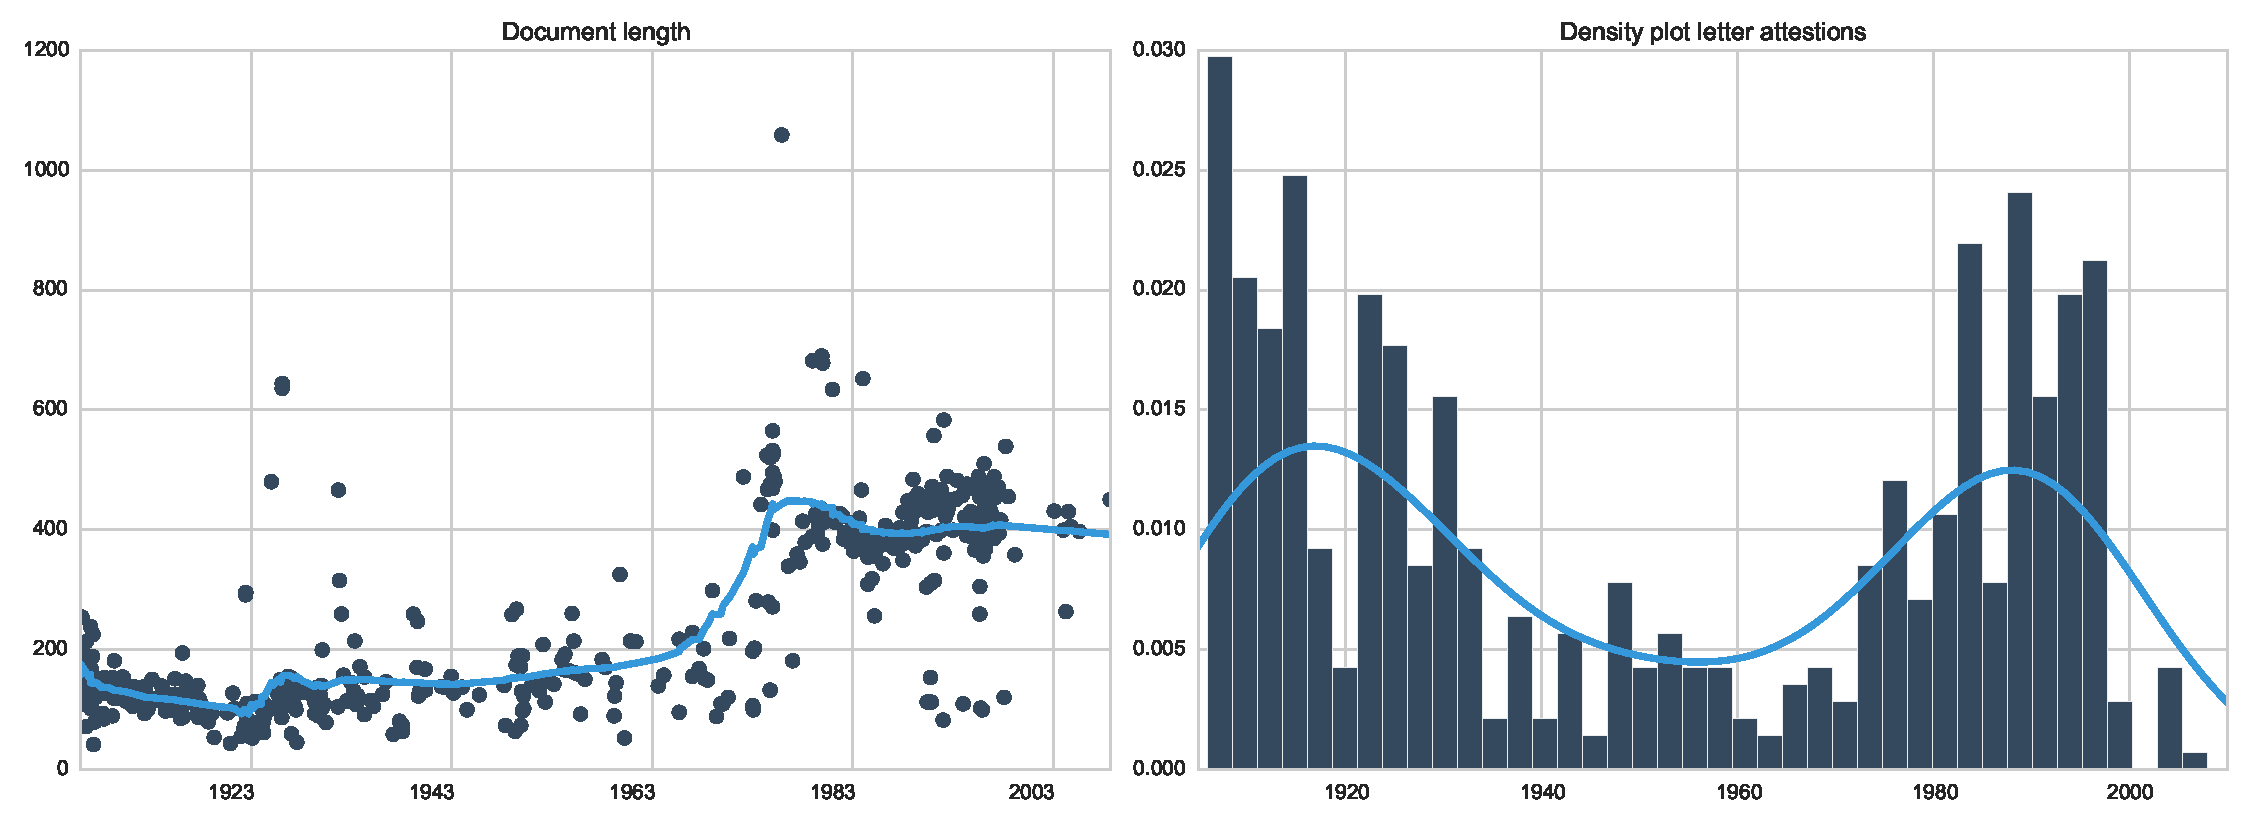
\includegraphics[width=\textwidth]{images/luck-statistics.pdf}
  \caption{Diachronic visualization of some general statistics about the Luck chain letter corpus. The left subplot visualizes the letter length (expressed in word forms), and the right subplot shows a kernel density plot of the number of letters attested per year.}
  \label{fig:luck-statistics}
\end{figure}

For this study, I constructed a full-text version of the Luck chain letter collection\autocite{folgert_karsdorp_2016_51588}. The total number of letters in this version of the collection amounts to 554. The oldest letters stem from 1906 and the youngest from 2008. Each year in the collection is represented by six letters on average. The collection was tokenized using the tokenizer of the \emph{Natural Language Toolkit}~\autocite{bird:2009}. The total number of words amounts to 134,589 (including punctuation). In their lowercased form, 5,256 of these word forms occur uniquely. Letters consist of 243 word forms on average. Figure \ref{fig:luck-statistics} visualizes some general statistics of the corpus. The left subplot visualizes how the letter length changes over time. It can be observed that until the 1980s the letter length has remained generally stable over time. Around 1980 the letters suddenly become significantly longer, which might reflect some severe changes to the tradition that require further investigation. The right subplot shows the density with which letters have been attested each year. Most letters stem from either the beginning or from the last two decades of the \nth{20} century. 

\section{Story Network Construction}\label{sec:networks}

Story networks consist of stories and links between stories that represent pre-textual relationships. In this study, I make the simplifying assumption that stories that are more similar to each other are more likely to stand in a pre-textual relationship than stories that are more distant. In what follows, I discuss a vocabulary-based representation of stories, the `bag-of-words' representation, that is suitable for computational methods of discovering textual similarity. Subsequently, in Section \ref{sec:bootstrapping-networks} I present a clustering algorithm that aims to bootstrap pre-textual relationships between stories from raw collections of texts. Next, I describe how story networks are constructed on the basis of the output of this clustering procedure. Finally, I present the network-theoretic statistics to detect and describe pre-textual relationship characteristics of story networks in Section \ref{sec:construction-statistics}.

\subsection{Bag-of-Words Models}

Bag-of-words models have proven to be invaluable for numerous computational approaches to textual data, such as text classification, textual information retrieval and textual stylometry. Bag-of-words models make the assumption that maintaining word order is unnecessary in determining the relationship between texts. Obviously, this is a crude simplification, yet there is a surprising number of applications in which word order adds barely any additional information. Given a corpus $C$ consisting of a vocabulary $V$ (i.e.\ word types), bag-of-words models represent documents as histograms over the vocabulary, that is, as vectors of occurrence counts of words. For a document $d$, the vector representation $\mathbf{w}^{(d)}$ is given by $(w_1, w_2, \ldots, w_V)$, where $w_i$ represents the occurrence counts of word $i$ in document $d$. Consider the following vocabulary: $\{\textit{story, dialogue, network, reader, model}\}$. Each word in the vocabulary is represented by a unique integer: $\{1, 2, 3, 4, 5\}$. A document $d$ that consists of the words ``\emph{model, network, network}'' can then be represented by the following vector: $\mathbf{w}^{(d)} = (0, 0, 2, 0, 1)$. 

It is common practice in many computational applications to weigh the word frequency vectors for term importance. Here, I make use of the well-known `term frequency-inverse document frequency' (tf-idf) weighting scheme, which weighs the frequency of words in a document (tf) against the background of how many documents in the collection contain those words (idf)\autocite{manning:2008}. The transformed vectors put more weight on words that occur relatively often in a particular document (i.e.\ their term frequency is high) and relatively rarely in the corpus as a whole (i.e.\ their document frequency is low). Words with high weights can be considered to be topical words that represent the contents of a text. Words with low values occur either too often in the corpus or too rarely in the document to be of topical value to a document. 

Using these vector representations, the similarity (or distance) between two stories can be assessed by means of a pairwise comparison of their vector values. I choose to use the Cosine dissimilarity measure to express the distance between two stories in terms of their weighted occurrence count vectors. Given two story vectors $\mathbf{a}$ and $\mathbf{b}$, the Cosine dissimilarity can be computed using the following expression:
\begin{equation}
\delta_C(\mathbf{a}, \mathbf{b}) = 1 - \frac{\sum^V_{i=1} a_i \times b_i}{\sqrt{\sum^V_{i=1} (a_i)^2} \times \sqrt{\sum^V_{i=1} (b_i)^2}}
\end{equation}
where $a_i$ represents the weighted count of word $i$ in vector $\mathbf{a}$ and $b_i$ the weighted count in vector $\mathbf{b}$.


\subsection{Bootstrapping Pre-textual Relationships}\label{sec:bootstrapping-networks}

Given a story, how can we identify a set of potential pre-texts $P$ from a collection of stories $C$? Using the story representation discussed in the previous section, we can compute the distance between a story $i$ attested at time $t_i$ and all potential pre-texts. Like in Chapter \ref{chp:red-riding-hood}, stories are considered to be potential pre-texts if and only if they are attested prior to $t_i$, that is $P = \{j | \forall j \in \{1, 2, \ldots, C\} \wedge t_j \leq t_i \wedge i \neq j\}$, where $C$ represents the complete set of stories in the collection. This set of potential pre-texts can then be sorted in ascending order to obtain a ranking in which the top items represent the most like pre-texts of story $i$. 

We can apply a cutoff to these rankings to assign to each story its $k$ most likely pre-texts. At a cutoff of $k=1$, we only take into consideration the most similar (or least distant) text, whereas at $k=|P|$ the complete set of potential pre-texts is taken into account. Unfortunately, it is not straightforward to define the value $k$ in a non-arbitrary way. A more fundamental problem of this approach, however, is the possibility that the set of potential pre-texts does not contain an actual pre-text in the first place. In the most extreme case, the most similar pre-text ($k=1$) is maximally distant from the story under consideration. A possible way to overcome this problem is to define a threshold value at which stories are considered to be too distant to be related. The exact value of this threshold, however, is sensitive to a multitude of factors, such as the corpus under investigation, its feature representation, and the distance metric used. 

The problem we face is essentially an open-set problem: given as set of potential pre-texts, can we decide which of them are similar enough to be considered actual pre-texts of a particular story? This includes the possibility that \emph{none} of the potential pre-texts are similar enough. The problem as formulated here is closely related to the \emph{many candidates} problem in the context of authorship verification\autocite{koppel:2014}. In that problem, the goal is to assess whether the author of some anonymous document is someone among a set of candidate authors, or a yet unknown author\autocite{koppel:2014}. To overcome the sensitive practice of defining ranking cutoff values or distance thresholds, I will describe a procedure that allows us to exclude potential pre-texts from consideration in a more robust and less arbitrary way. The procedure draws inspiration from resampling methods\autocite{good:2006} and methods proposed to tackle the author verification problem\autocite{koppel:2014}.

\begin{algorithm}[t]
\KwData{story $i$, pre-texts $P = \{j | \forall j \in \{1, 2, \ldots, C\} \wedge t_j \leq t_i \wedge i \neq j\}$}
$S \leftarrow $ an array of size $|P|$ with assignment counts for each pre-text\;
$A \leftarrow \emptyset$\;
\For{iteration $t \leftarrow 1$ \KwTo $T$}{
  $P^{(t)} \leftarrow$ construct a new representation of $P$ based on a random sample (e.g.~50\%) of the complete feature space\;
  $j \leftarrow \argmin_{j \in P^{(t)}} d_C(i, j)$\;
  $S_j \leftarrow S_j + 1$\;
}
\For{pre-text $j \leftarrow 1$ \KwTo $|P|$}{
  \If{$\frac{1}{T} S_j > \sigma$}{
     $A \leftarrow A \cup \{j\}\;$
  }
}
\Return{A}
 \caption{Bootstrap Neighbor Clustering}
 \label{alg:boostrap-clustering}
\end{algorithm}

The general idea behind the procedure is to assess the rankings of pre-texts for their robustness by approaching the data from various angles for a large number of trials. If we compute the distances between a story and its potential pre-texts on the basis of a slightly modified feature space (i.e.\ we leave out a small number of words from the bag-of-words representation), we want the resulting rankings to be consistent with those of the unmodified feature space. We repeat this process and in each trial we compute the distances between each story and its potential pre-texts on the basis of a random sample (e.g.~50\%) of the complete feature space. Each trial potentially produces slightly (or very) different rankings. We select from each trial the $k=1$ nearest neighbor for each story and compute the fraction of trials $\mu$ that this potential pre-text was identified as the most similar (or least distant) story. The result of the procedure is a ranking of potential pre-texts for each story $i$ in which the positions represent the consistency with which pre-texts have been identified as the nearest neighbor of $i$ over all trials. Some stories unequivocally select the same nearest neighbor over all trials ($\mu=1$), whereas for others the selection is more ambiguous, e.g.\ the most consistent selection does not exceed 20\% of the trials ($\mu=0.2$). Depending on how conservative one wants the selection to be, a fixed cutoff value can be used that expresses the lower bounds of the fraction of trials with which a pre-text has to selected as the nearest neighbor of a story. At $\mu=0$ all potential pre-texts are selected, whereas $0.5 < \mu \leq 1$ maximally returns one nearest neighbor. In the experiments below, $\mu$ is set to the rather conservative value of 0.5. Algorithm \ref{alg:boostrap-clustering} summarizes the procedure, which I will refer to as \emph{Bootstrap Neighbor Clustering}.

\subsection{Story Networks and Statistical Methods}\label{sec:construction-statistics}

Given a bootstrapped set of pre-texts $A$ for story $i$, each pre-text selection is represented as a link using the following notation: $i \rightarrow j$ where $j$ refers to one of the pre-texts in $A$.\footnote{To avoid any misunderstandings, it should be stressed that we do \emph{not} treat stories and pre-texts as two separate classes, as any story can become a pre-text to a later story.} In network theory, these links are called directed edges between pairs of vertices. Consider the following set of stories, in which each number corresponds to a unique story: 
\begin{equation}
V = \{1, 2, 3, 4, 5\},
\end{equation}
The set  of pairs of stories and pre-texts is represented by: 
\begin{equation}
E = \{3 \rightarrow 2, 4 \rightarrow 3, 5 \rightarrow 3\}.
\end{equation}
Using $V$ and $E$ we create a graph $G = (V, E)$ that can be visualized as in Figure \ref{fig:example-network}. Note that in this hypothetical example, story 1 is a singleton story for which no decisive pre-text could be determined. 

\begin{figure}
\centering
\begin{tikzpicture}[shorten >=1pt,->]
  \tikzstyle{vertex}=[circle,text=white,fill=paperblue,minimum size=17pt,inner sep=0pt]
%%
\pgfsetcolor{papergray}
  % Edge: v1 -> v2
  % \draw [->] (110.89bp,96.315bp) .. controls (119.4bp,93.002bp) and (129.88bp,88.92bp)  .. (148.83bp,81.538bp);
  % Edge: v3 -> v2
  \draw [->] (110.89bp,53.586bp) .. controls (119.4bp,56.899bp) and (129.88bp,60.98bp)  .. (148.83bp,68.362bp);
  % Edge: v4 -> v3
  \draw [->] (36.99bp,68.315bp) .. controls (45.496bp,65.002bp) and (55.978bp,60.92bp)  .. (74.934bp,53.538bp);
  % Edge: v5 -> v3
  \draw [->] (36.99bp,25.586bp) .. controls (45.496bp,28.899bp) and (55.978bp,32.98bp)  .. (74.934bp,40.362bp);
  % Node: v1
  \node[vertex] at (92.851bp,102.95bp) {$1$};
  % Node: v2
  \node[vertex] at (166.75bp,74.95bp) {$2$};
  % Node: v3
  \node[vertex] at (92.851bp,46.95bp) {$3$};
  % Node: v4
  \node[vertex] at (18.95bp,74.95bp) {$4$};
  % Node: v5
  \node[vertex] at (18.95bp,18.95bp) {$5$};
%
\end{tikzpicture}
\caption{Artificial story network.}
\label{fig:example-network}
\end{figure}

The number of incoming edges (i.e.\ the number of stories that select a particular pre-text) is called \emph{in-degree}. I use the notation $d_{in}(i)$ to refer to the in-degree of node $i$. If we apply this terminology to the network in Figure \ref{fig:example-network}, we can observe that node 3 has an in-degree of $d_{in}(3) = 2$, whereas node 2 has an in-degree of 1. $Pr(d_{\text{in}})$ is used to refer to the in-degree distribution of a network. Node 1, 4 and 5 have an in-degree of 0. Node 2 has one incoming link ($d_{in}(2)=1$) and node 3 has two incoming edges. $Pr(d_{\text{in}})$ then represents the probability that a randomly chosen node from the network has a particular in-degree (e.g. $Pr(d_{\text{in}}=1)$ = (number of nodes with $d_{\text{in}}=1$) / (total number of nodes) = 0.2).

A common approach to characterize degree distributions is to fit the parameters of a probability density function. Many real-world networks such as the Word Wide Web network and (scientific) citation networks display a degree distribution with a so-called `heavy tail' in which a large proportion of the nodes have a small degree and only a few yet significant number of nodes are connected to many nodes\autocite{newman:2003}. In some networks the degree of the nodes decays exponentially, whereas in others it follows a power-law:
\begin{equation}\label{eq:powerlaw}
Pr(d) \approx d^{-\alpha}
\end{equation}
where values of the parameter $\alpha$ typically fall in the range $1.5 \leq \alpha \leq 3$\autocite[table II]{newman:2003}. Larger values lead to a faster decay in the probability of nodes with a high degree. To illustrate the effect of the exponent, I show in the left subplot of Figure \ref{fig:lorenz-examples} the complementary cumulative distribution function (ccdf) of four randomly generated degree distributions using different values of $\alpha$. Given that two degree distributions follow a power-law, we can compare the exponents of their distributions. However, as \citeauthor{clauset:2009} have shown, many empirical distributions that appear to follow a power-law, are in fact better described using other heavy-tail distributions such as the log-normal distribution\autocite{clauset:2009}. In this chapter, I apply the techniques developed by \citeauthor{clauset:2009} to characterize the degree distributions of story networks\autocite{clauset:2009}.

\begin{figure}
\centering
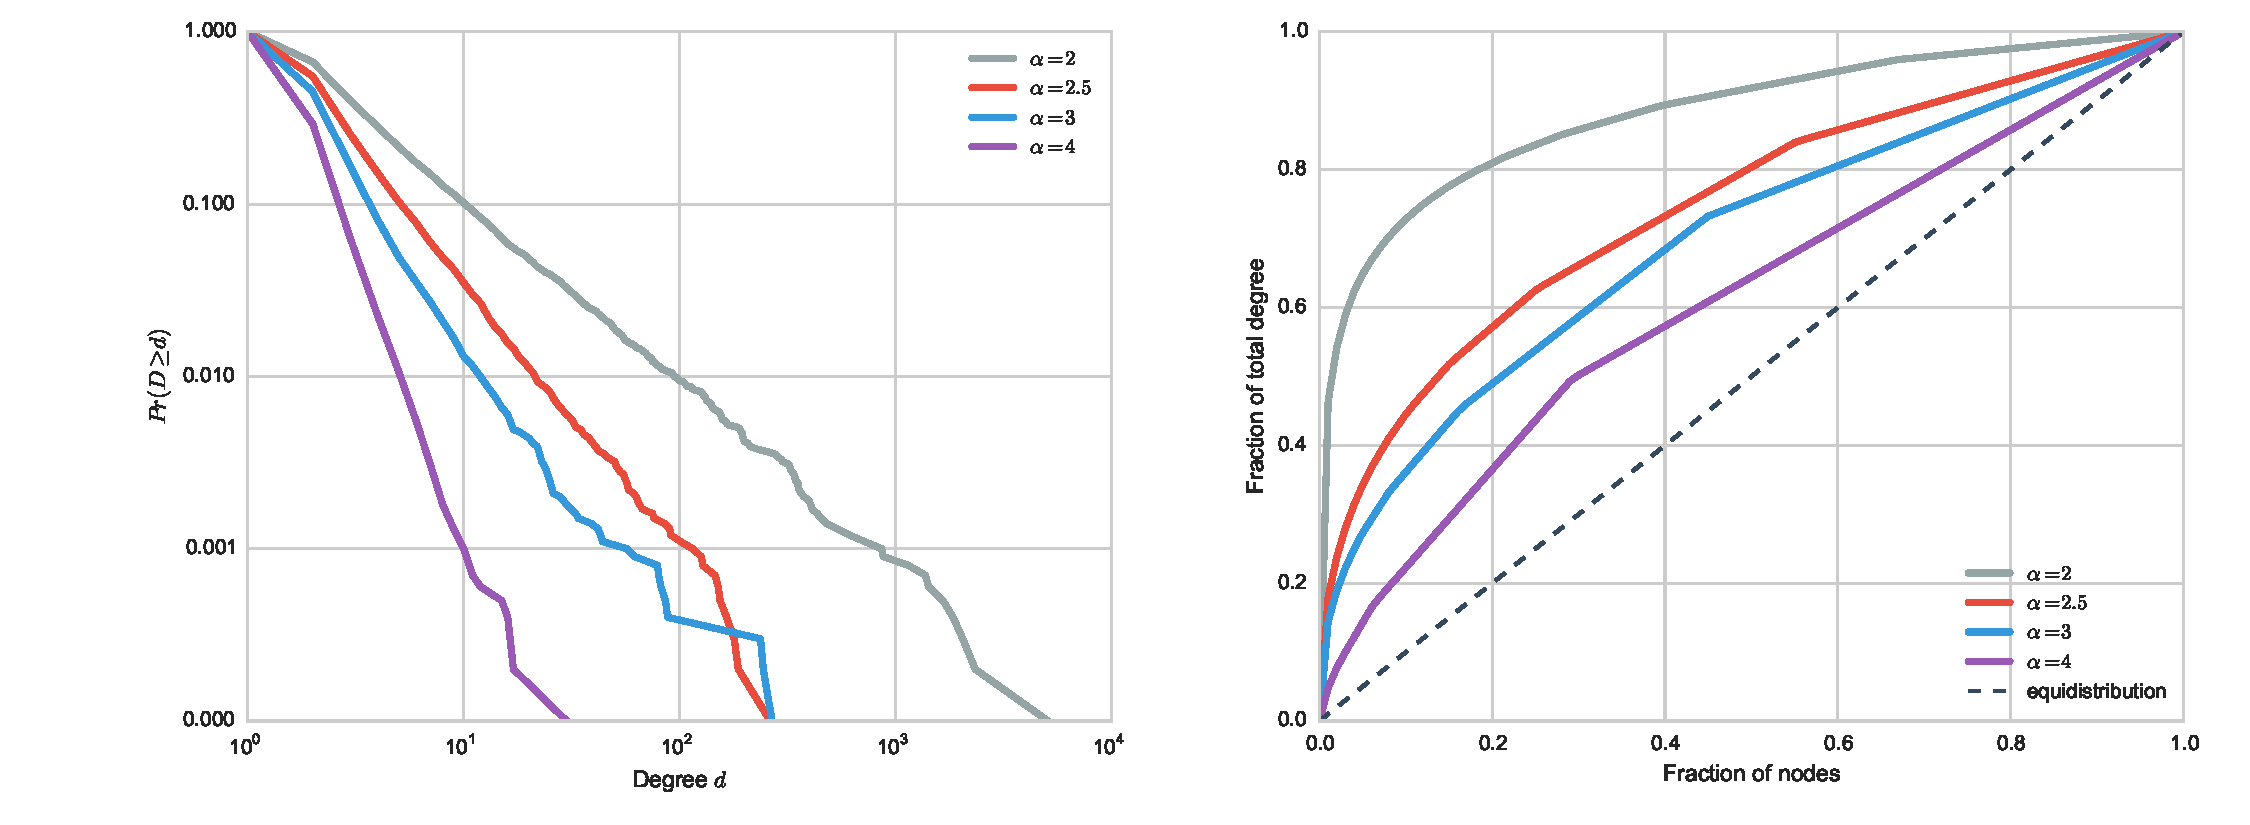
\includegraphics[width=\textwidth]{images/lorenz_examples.pdf}
\caption{Left: Complementary cumulative distribution functions of four power-law degree distributions with exponents of $\alpha=2$, $\alpha=2.5$, $\alpha=3$ and $\alpha=4$. Right: Lorenz curves corresponding to these power-law distributions. The dashed line represents a degree distribution that exhibits complete equality of the fraction of nodes over the fraction of degree.}
\label{fig:lorenz-examples}
\end{figure}

Heavy tails of degree distributions represent an uneven spread of edges among nodes. This inequality can be represented using a Lorenz curve which was developed by the economist Max Lorenz for representing wealth inequality in a population. The curve displays the fraction of wealth held by the richest fraction of people in a population. Applied to network degree distributions, the curves represent what fraction of edges is held by what fraction of nodes. If all nodes in a network are connected by the same number of edges, the curve forms a straight line, representing total equality. In the situation where a small fraction of nodes holds a large fraction of edges, the curve displays a steep increase, indicating that the edges are spread unevenly among the nodes. To illustrate the Lorenz curve, I show in the right subplot of Figure \ref{fig:lorenz-examples} the Lorenz curves of the degree distributions that correspond to the power-law exponents in the left subplot. The dashed line represents a degree distribution that exhibits complete equality of the fraction of nodes held by the fraction of edges. The degree distribution generated using $\alpha=2$ displays the strongest form of inequality in which only a small fraction of the nodes (0.2) holds a large fraction of the edges (0.8).

The degree of inequality observed in Lorenz curves can be conveniently summarized using the Gini coefficient $G$. This coefficient can be defined as twice the area between the equidistribution (i.e.\ the dashed line in Figure \ref{fig:lorenz-examples}) and an observed Lorenz curve. $G$ falls in the range $0 \leq G \leq 1$ where larger values indicate a higher degree of inequality. The Lorenz curve corresponding to the degree distribution generated with $\alpha=4$ yields $G=0.22$, whereas the curve corresponding to $\alpha=2$ is summarized by $G=0.77$. An advantage of the Gini coefficient is that it allows us to compare networks of different average degree and size\autocite{Badham:2013}. 


\section{Story Network Analysis}\label{sec:network-analysis}

\begin{sidewaysfigure}
\centering
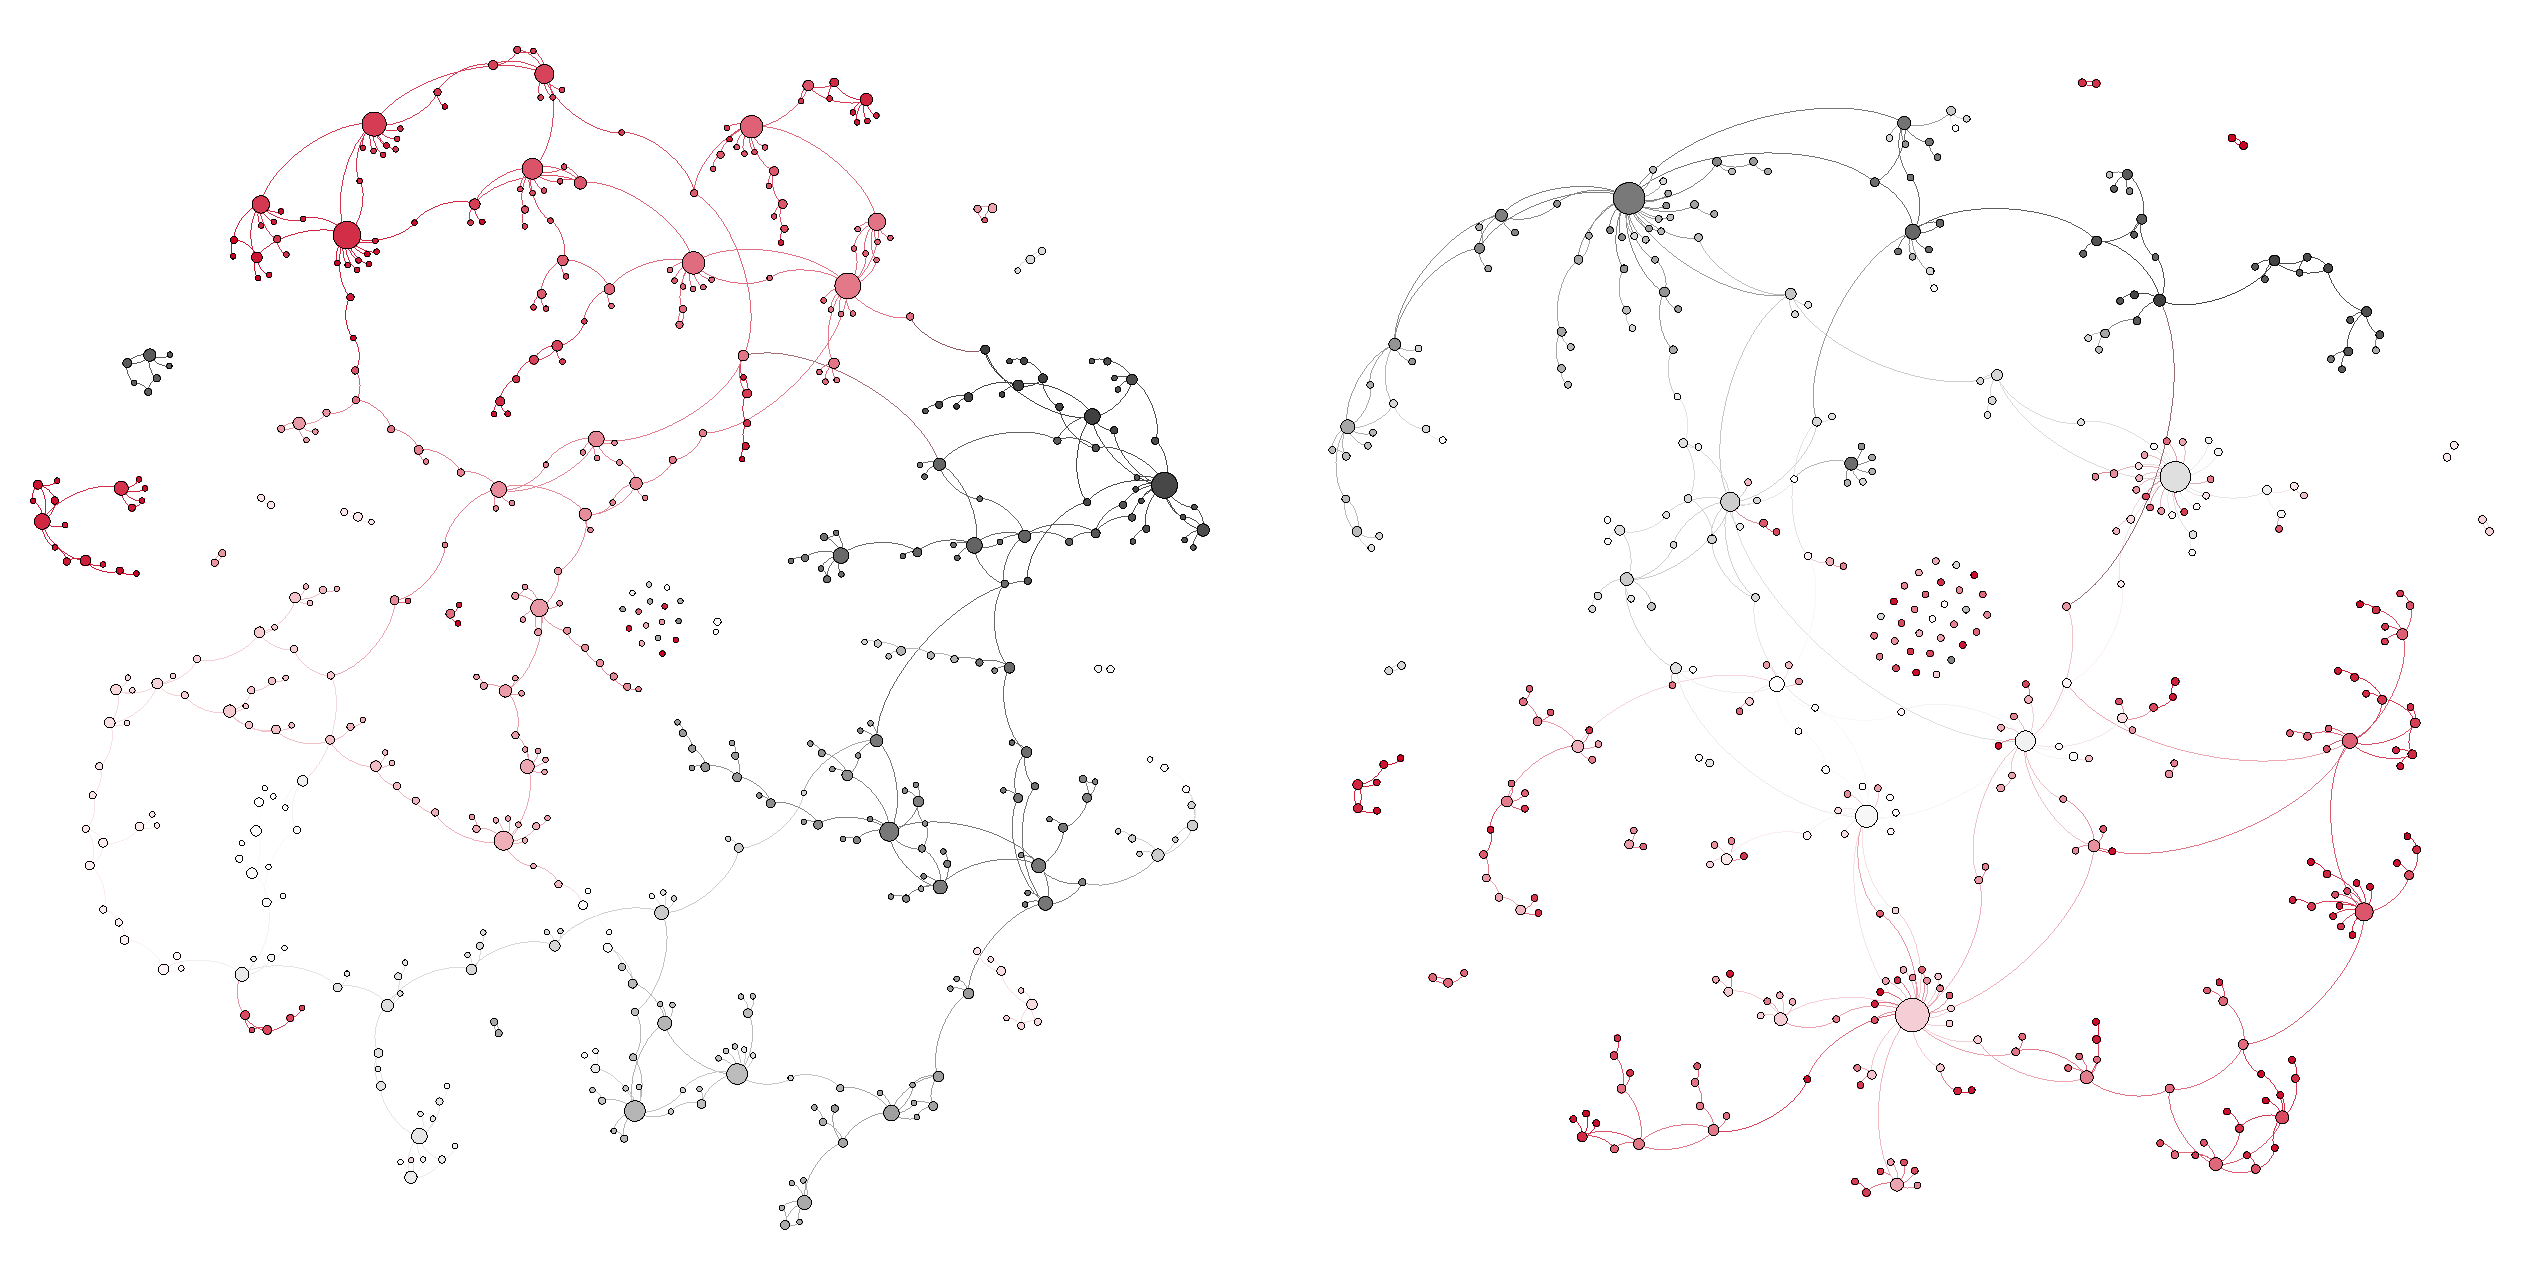
\includegraphics[width=\textwidth]{images/graphs.pdf}
\caption{Story networks of the collection of chain letters (left network) and ``Red Riding Hood'' retellings (right network). Nodes represent individual stories and edges represent pre-textual relationships between stories. The color gradient (from black via white to red) represents the age of each story.}
\label{fig:network-visualization}
\end{sidewaysfigure}

To construct story networks for the collection of ``Red Riding Hood'' retellings and the collection of chain letters, I employ the \emph{Bootstrap Neighbor Clustering} procedure. Figure \ref{fig:network-visualization} provides a graphical visualization of the two networks. The ``Red Riding Hood'' network consists of $n=427$ nodes and $m=439$ edges. The chain letter network consists of $n=554$ nodes and $m=620$ edges. The color gradient (from black via white to red) in the two networks represents the age of each story. Two important observations can be made from visually inspecting the two networks. First, let us consider the chain letter network. As indicated in the introduction and data section, chain letters are explicitly designed to be replicated and redistributed within a short period of time. To confirm the reliability of the proposed methodology, then, the story network extracted by the \emph{Bootstrap Neighbor Clustering} procedure has to be in accordance with some of our preconceptions about the structure of chain letter story networks. The visualization in Figure \ref{fig:network-visualization} indicates that this appears to be the case: most stories in the network are connected to other stories with a similar color shade, which means that, in the chain letter network, stories predominantly select stories of approximately the same age as potential pre-texts. Interestingly, the second (``Red Riding Hood'') network exhibits a similar pattern, with each story showing a clear preference to select pre-texts with a similar color shade (i.e.\ close temporal proximity). Second, it can be observed that the network derived from ``Red Riding Hood'' retellings has a structure with a few hubs, i.e.\ where three or four stories function as pre-text for a large number of stories (which is represented by the size of the nodes in the networks). The chain letter network, on the other hand, displays a more uniform distribution over which stories function as pre-text, which also is in accordance with our expectations about the structure of chain letter networks (cf.\ Section \ref{sec:networks-introduction}).

In what follows, I will statistically characterize these two observations by carefully studying the in-degree distributions of the two story networks. Accurately characterizing the in-degree distribution of the two networks is a fundamental prerequisite to understand which models of network growth potentially underlie the evolution of the two story networks. A power-law characterization of the in-degree distribution, for example, might be accounted for by models of network growth such as the Preferential Attachment model (cf.\ Section \ref{sec:network-evolution}). Subsequently, I will study the development of the two story networks over time. I compare four models of network growth and analyze their in-degree distributions in relation to those of the two story networks.

\subsection{In-Degree Distribution Analysis}

Figure \ref{fig:degree-fits} plots the cumulative complementary distribution function (ccdf) of the in-degree distributions of the story networks on doubly-logarithmic axes. The plots express the probability of stories with at least in-degree $d_{\text{in}}$, which is denoted as $Pr(D \geq d_{\text{in}})$, where $D$ represents a random variable drawn from the distribution. The plots clearly show that the vast majority of stories have a small in-degree and that only a few stories are selected as pre-text by a large(r) number of stories. 

\begin{figure}[t]
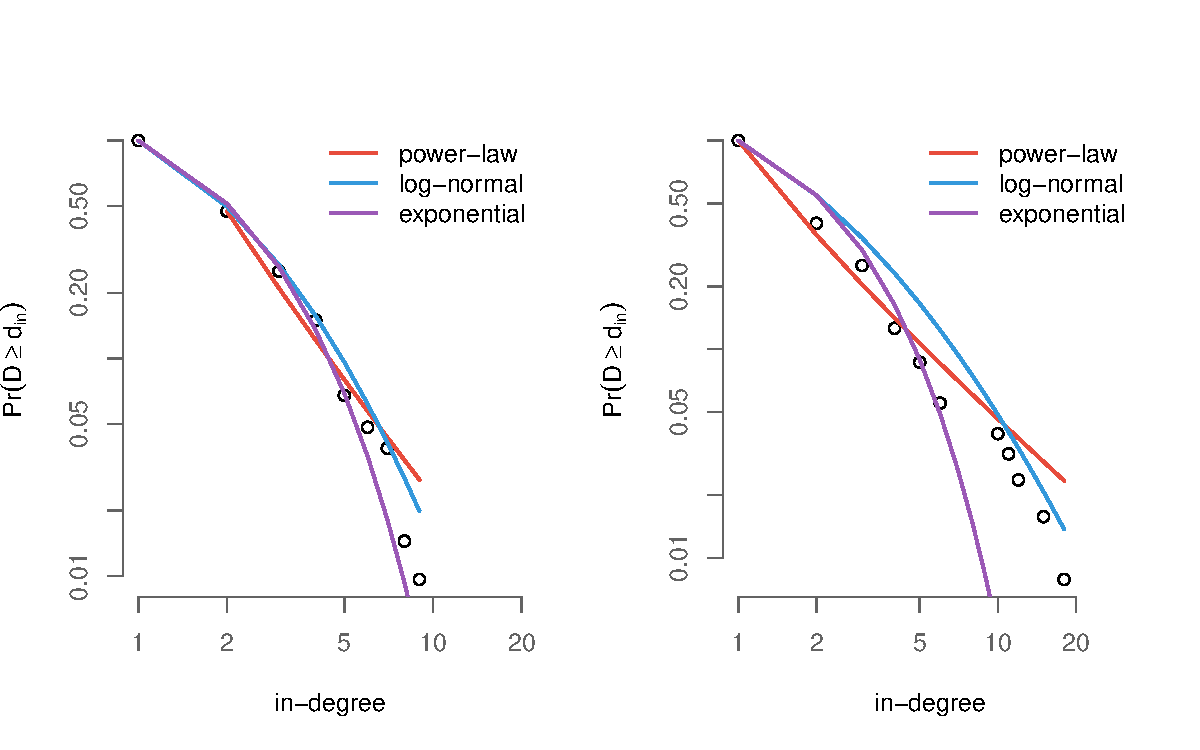
\includegraphics[width=\textwidth]{images/degree-fits.pdf}
\caption{Complementary cumulative in-degree distributions of the two story networks (left: chain letters; right: ``Red Riding Hood''). The plot provides for both distributions the best fit of a power-law, log-normal and exponential model. The power-law and log-normal model both fit the empirical in-degree distribution of ``Red Riding Hood'' well. The chain letter in-degree distribution is best described by means of an exponential model.}
\label{fig:degree-fits}
\end{figure}

To obtain a better understanding of the distributions, I perform the rigorous statistical procedure as described by \citeauthor{clauset:2009} to detect power-law behavior in distributions\autocite{clauset:2009}. In many real-world datasets, the power-law property only applies to the tail of the distribution, i.e.\ for values greater than some minimum value $d_{\text{min}}$. The method proposed by \citeauthor{clauset:2009} estimates a minimum value $d_{\text{min}}$ by comparing the empirical distribution to the theoretical cumulative distribution function (cdf). The method aims to optimize the Kolmogorov-Smirnov statistic $D$ by choosing $d_i$ as the value for $d_{\text{min}}$ for which $D$ is the smallest. \citeauthor{clauset:2009} suggest to test whether a dataset actually follows a power law using a goodness-of-fit test and a bootstrapping procedure\autocite{clauset:2009}. The $p$-value resulting from this test answers the question whether possible differences between the empirical data and the model are significant or not. If $p \simeq 0$, then the model cannot be deemed a plausible fit and other distributions are more appropriate. 

At a significance level of 95\%, we cannot reject the hypothesis that the in-degree distribution of the ``Red Riding Hood'' network is generated by a power-law model: $D=0.048, p > 0.07$. By contrast, the power-law model is not a good fit for the in-degree distribution of the chain letter network ($D=0.09, p = 0.001$). Another way to test for power-law behavior is to directly compare a power-law model to another model, such as a log-normal model via a \emph{likelihood ratio test} $R$\autocite{clauset:2009}. Using the likelihood ratio test, we can assess whether the in-degree distributions are more appropriately described by means of a log-normal or exponential model. The log-normal model fits the chain letter distribution significantly better than the power-law model for the full range of in-degree values ($TS=-4.05, p < 0.0001$). The next step is to compare the log-normal model to an exponential model. The test results are indecisive as to whether a log-normal model is more appropriate than an exponential model ($R=0.079, p > 0.9$). Since a log-normal function has more parameters than an exponential function, it seems reasonable -- for reasons of parsimony -- to characterize the chain-letter in-degree distribution as exponential. Although a log-normal model appears to fit the in-degree distribution of ``Red Riding Hood'' slightly better than a power-law function, the test results suggest that the two models do not perform \emph{significantly} different ($R=-1.52, p > 0.1$).

\begin{figure}
\centering
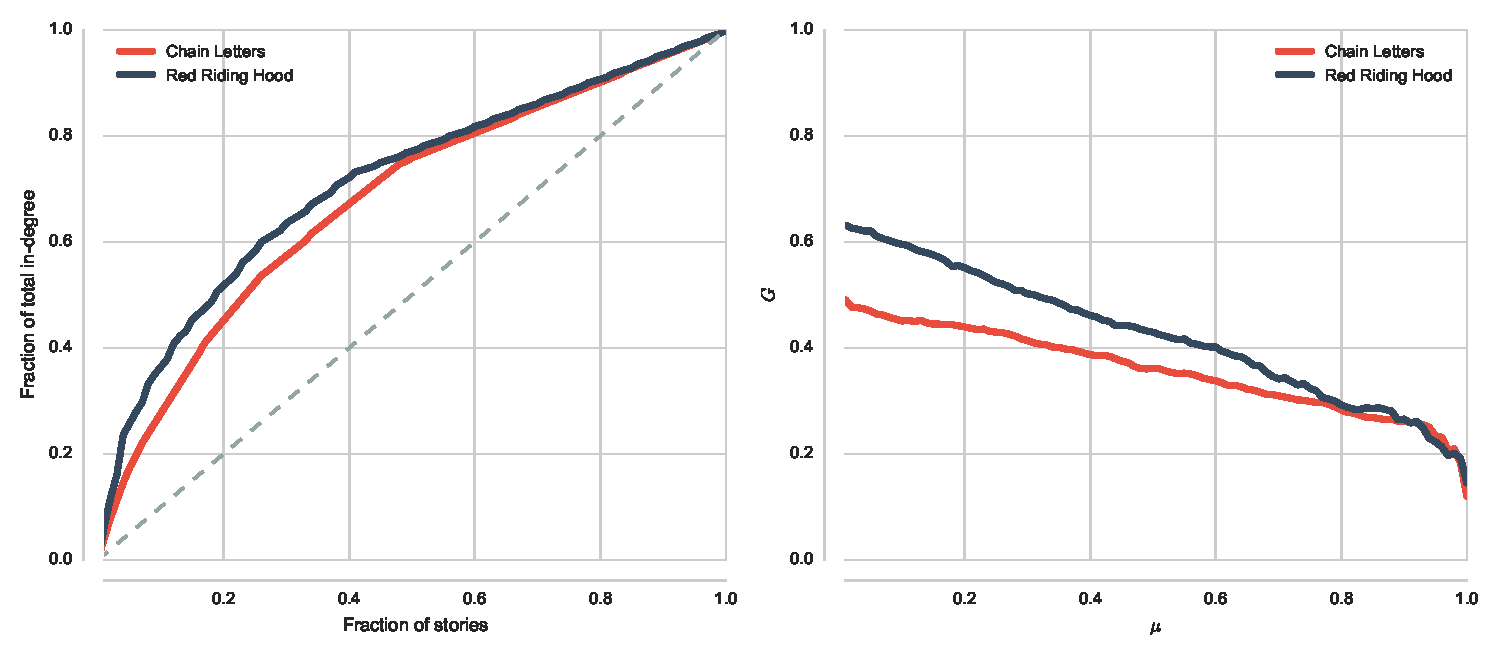
\includegraphics[width=\textwidth]{images/gini-lorenz.pdf}
\caption{The left subplot displays the Lorenz curve of the chain letter and \emph{Red Riding Hood} story network. The gray striped line represents the equidistribution. The right subplot shows the Gini coefficient $G$ of the in-degree distributions for story networks constructed using $\mu$ in the range $0.1 \leq \mu \leq 1$. It can be observed that the value of $G$ remains relatively stable as we increase the value of $\mu$.}
\label{fig:degree-statistics}
\end{figure}

In the left subplot of Figure \ref{fig:degree-statistics}, I present the Lorenz curves of the two in-degree distributions. The summarizing Gini coefficients of these curves are $G=0.36$ for the chain letter network and $G=0.43$ for ``Red Riding Hood''. Compared to their random counterparts, the story networks exhibit a greater degree of inequality with respect to their in-degree distributions (chain letters: $G_{\text{random}}=0.3$; ``Red Riding Hood'': $G_{\text{random}}=0.28$).\footnote{These random graphs are created by randomly rewiring the edges of the story networks while preserving the time constraint, i.e.\ stories may only link to randomly chosen pre-texts of the same or older age.} The degree of inequality is especially large in the case of ``Red Riding Hood'', suggesting that relatively few stories function as pre-text for many other stories. In the right subplot of Figure \ref{fig:degree-statistics}, I visualize the Gini coefficients $G$ for story networks that were constructed with $0.1 \leq \mu \leq 1$. It can observed that the in-degree distributions display a relatively uneven spread of edges among nodes (i.e.~stories) even for high values of $\mu$. This indicates that the `hubness' of the networks is a stable characteristic and not too much the result of cherry picking a particular value of $\mu$. 


\subsection{Story Network Evolution}\label{sec:network-evolution}

In the previous section, I have shown that the two studied story networks display distinct in-degree distributions. The chain letter network exhibits an in-degree distribution which decays exponentially. The ``Red Riding Hood'' network, by contrast, exhibits a heavy-tail in-degree distribution that fits a power-law or log-normal model reasonably well. Retellings of ``Red Riding Hood'' preferentially link to a small number of stories that are pre-texts of many other retellings. In the present section, I turn to the central question of how these distributions come into being. By carefully studying and comparing the structure and evolution of the two story networks to formal models of network growth, I provide empirical evidence for three major conclusions regarding the formation of story networks. First, I provide empirical evidence that stories preferentially select stories in close temporal proximity, which is indicated by a strong lopsidedness towards smaller time-spans in the time-span distributions of stories and their selected pre-texts. Second, I show that the in-degree distribution of the ``Red Riding Hood'' network is significantly correlated with the age of stories, suggesting that retellings of ``Red Riding Hood'' are affected by a mechanism of preferential attachment in which slightly older versions are preferred to be selected as pre-text(s) in producing a new version. Finally, I show that stories have individual attractiveness values that lessen over time.

The Preferential Attachment (PA) model has proven to be a reliable model to account for heavy-tail degree distributions observed in real-world networks. The model was invented by Derek de Solla Price in the context of citation networks\autocite{price:1976} and simplified and generalized by Albert-László Barabási and Réka Albert to account for undirected networks\autocite{barabasi:1999}. The algorithm generates these networks using an attachment mechanism in which new nodes preferentially link to existing nodes with high (in-)degree. A social network is a classic example in which the mechanism of preferential attachment is at play. In a social network, an edge between two persons $a$ and $b$ exists if $a$ knows $b$ or vice versa. Some persons have many connections and a newcomer to the network is more likely linked to these well-known persons than to persons who are relatively unknown. Similarly, web pages preferentially link to well-known sites, such as Wikipedia, rather than to sites that are less familiar. The mechanism of preferential attachment predicts that the probability of creating a new link between entity $a$ and $b$ is proportional to the number of existing connections of $b$. 

\begin{figure}
\centering
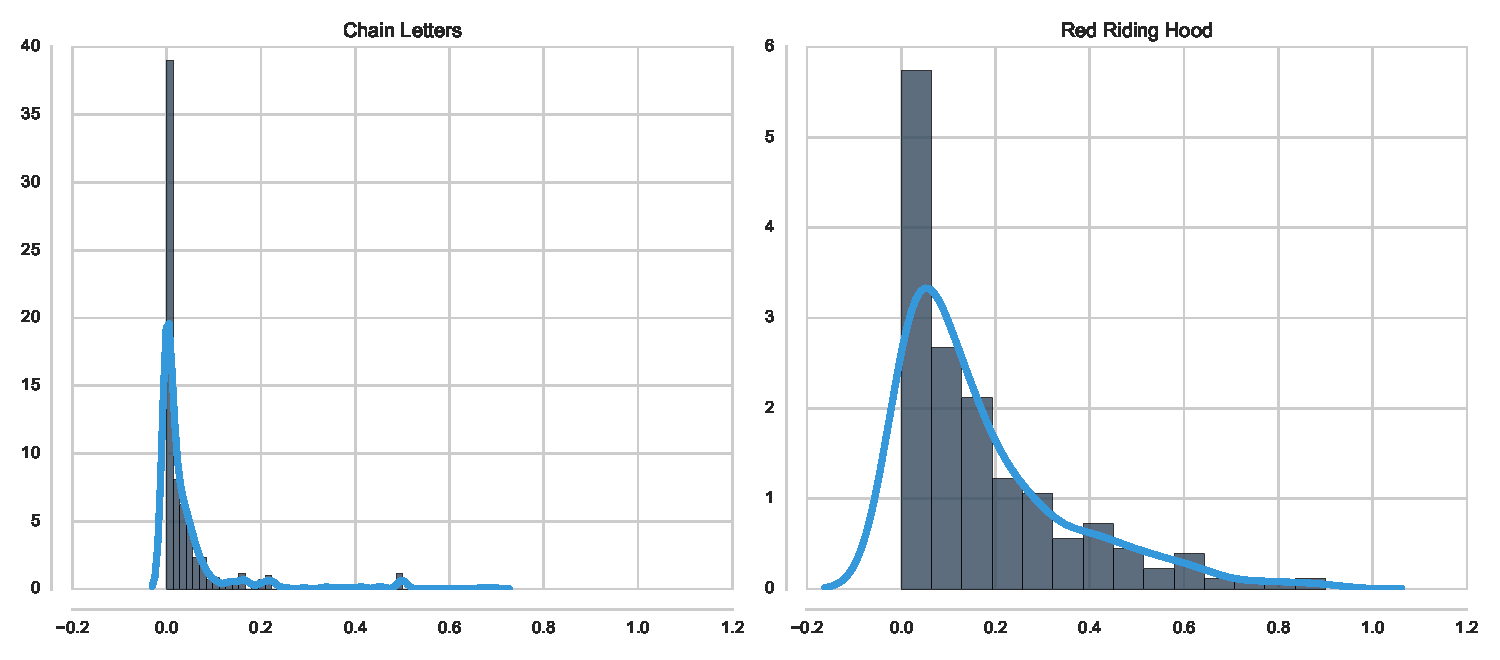
\includegraphics[width=\textwidth]{images/attachment.pdf}
\caption{Kernel density plots of time-span distributions. The plots display the distributions over time-spans for the chain letter network and the network induced for Red Riding Hood. As can observed, both time-span distributions display a strong lopsidedness towards smaller time-spans, which indicates a preference for pre-texts in close temporal proximity.}
\label{fig:time-attachment}
\end{figure}

The consequence of the preferential attachment mechanisms is that nodes that enter the network first will attract more links early on, and will continue to do so. As an explanatory model for story networks, the PA model predicts that stories preferentially select old(er) stories as pre-text rather than new(er) stories. To test this hypothesis, I evaluate for each pair of story and pre-text the time elapsed between their publication dates. Figure \ref{fig:time-attachment} plots the kernel density plots of the time-span distribution for the chain letter network and the ``Red Riding Hood'' network. The time-spans have been normalized to $0 \leq \tau \leq 1$, where $\tau$ represents the normalized time-span between a story and a pre-text. Both plots display strong lopsidedness towards smaller time-spans. Chain letters display an even stronger preference for pre-texts in close temporal proximity (median $\hat{\tau}=0.01$) than the retellings of ``Red Riding Hood'' (median $\hat{\tau}=0.11$). Both time-span distributions run counter the prediction of the PA model that stories are predominantly connected to old(er) stories. 

To obtain more insight into the relation between the in-degree and time-span distributions of the story networks, I test in Figure \ref{fig:correlation-degree-age} for the correlation between in-degree and age. As can be observed from the left subplot and confirmed by a Pearson $\rho$ correlation test, there is no evidence that the in-degree distribution of the chain letter network depends on the age of stories ($\rho=-0.02, p > 0.6)$. However, the in-degree distribution of ``Red Riding Hood'' retellings (right subplot in figure \ref{fig:correlation-degree-age}) is significantly correlated with age ($\rho=0.27, p < 0.0001$). In other words, retellings of ``Red Riding Hood'' do display a preference to select older versions as their pre-text(s). Note, however, that although the correlation is significant, its coefficient is rather low and the relatively low slope of the linear fit suggests that age affects in-degree only in a limited, upper-bounded range.

\begin{figure}
\centering
\subfigure[Chain letters]{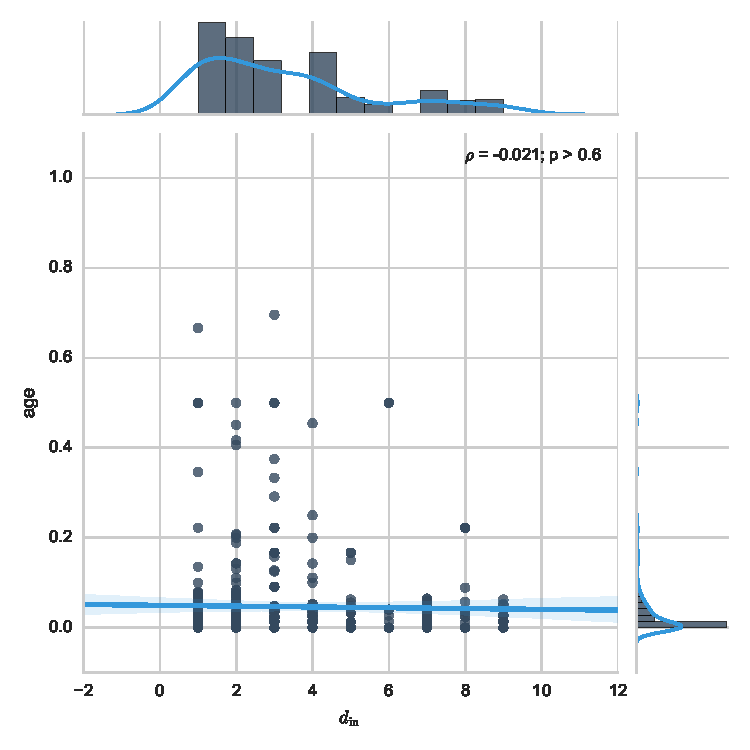
\includegraphics[width=0.49\textwidth]{images/letter-time-plot.pdf}}
\subfigure[``Red Riding Hood'']{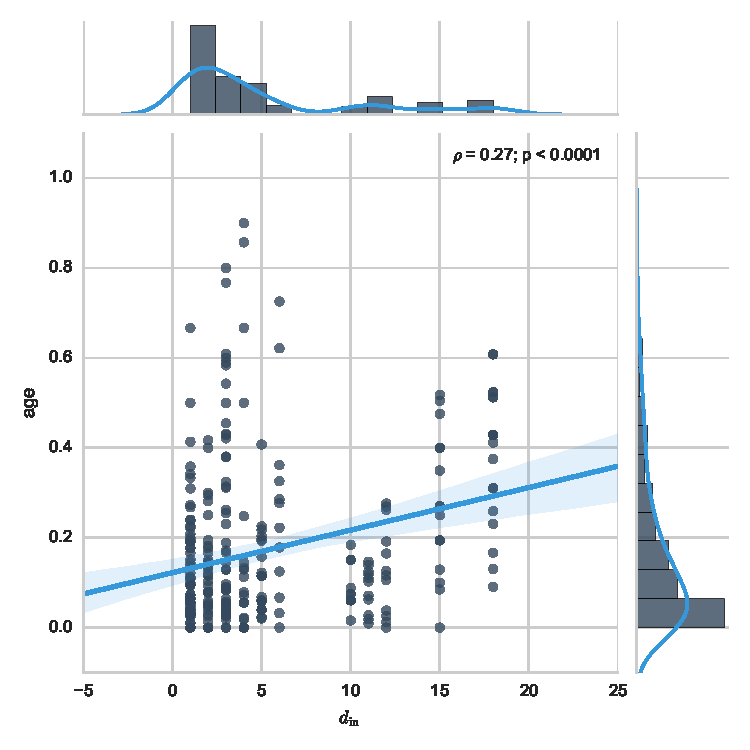
\includegraphics[width=0.49\textwidth]{images/rrh-time-plot.pdf}}
\caption{Correlation between in-degree and age. The two plots display the correlation between the age of a story and its in-degree for both the chain letter network and the ``Red Riding Hood'' network. The chain letter in-degree distribution does significantly correlate with the age of the letters ($\rho=-0.02, p > 0.6$). The in-degree distribution of the network of ``Red Riding Hood'' is significantly correlated with age ($\rho=0.27, p < 0.0001$).}
\label{fig:correlation-degree-age}
\end{figure} 

To account for the interaction between in-degree and age, I propose a growing network model, which is based on Price's model of preferential attachment~\autocite{price:1976}. In addition to the frequency-based attraction resulting from the preferential attachment mechanism, stories in this new model have individual values of attraction which lessen over time\autocite[Cf.][]{dorogovtsev:2000,eom:2011,Goldberg:2015}. Similar to the preferential attachment algorithm, the model begins with initializing an unconnected network consisting of $m_0$ nodes. At each succeeding time step a single node is added to the network. With a probability $(1 - p)$, a new node connects to $m \leq m_0$ existing nodes with uniform probability. With a probability $p$, the node is connected to $m \leq m_0$ nodes according to the preferential attachment mechanism. The probability to connect to an existing node is given by:
\begin{equation}
p(i) = \frac{\alpha_i \beta_i}{\sum^n_{j=1} \alpha_j \beta_j},
\end{equation}
where $\alpha_i = d_{\text{in}}(i)$ and $\beta_i$ represents the attractiveness of a node at a particular time step. If we set $\beta_i$ to represent a constant value, the model reduces to the original preferential attachment algorithm. Following previous studies\autocite[E.g.][]{eom:2011,Goldberg:2015}, I propose to lessen the attractiveness of a node exponentially over time:\autocite[Eom \& Fortunato add a node's in-degree to its attractiveness at a particular time step. In this study, I choose to weigh a node's in-degree by its attractiveness by \emph{multiplying} the two values. Cf.][]{eom:2011}
\begin{equation}
\beta_i = \beta^i_0 e^{- \tau / \gamma},
\end{equation}
where $\beta^i_0$ represents a node's initial attractiveness and $\tau$ represents the age of a node. The parameter $\gamma$ acts as an ``attention span'' parameter which controls the slope of the exponential decay\autocite{Goldberg:2015}. If $\alpha_i$ is held constant, the model's growth mechanism is restricted to the temporal attractiveness of nodes. Each node $i$ is assigned an individual initial attractiveness value $\beta^i_0$, which is sampled from a symmetric Dirichlet distribution with hyper-parameter $\phi$.\footnote{The choice for sampling from a Dirichlet distribution is largely motivated by the fact that Dirichlet processes are often employed to model data that, like the presented story networks, tend to develop in a `rich get richer' fashion.} Values of $\phi$ between zero and one generally result in a more `peaky' attractiveness distribution, in which only a few nodes are highly attractive. Higher values ($\phi \geq 1)$ result in a more uniform attractiveness distribution. In all experiments, I fix $\phi$ to 0.1. By holding the variable $\alpha_i$ and $\beta_i$ constant, we can analyze the various types of attractiveness in isolation and their interplay. More specifically, I investigate the following four models of network growth:
\begin{enumerate}
\item Preferential Attachment (PA) Model, where $\beta_i = 1$;
\item Temporal Preferential Attachment (T-PA) Model, where $\beta^i_0 = 1$;
\item Temporal Attractiveness (TA) Model, where $\alpha_i = 1$;
\item Preferential Attachment Temporal Attractiveness (PA-TA) Model.
\end{enumerate}

\begin{figure}
\centering
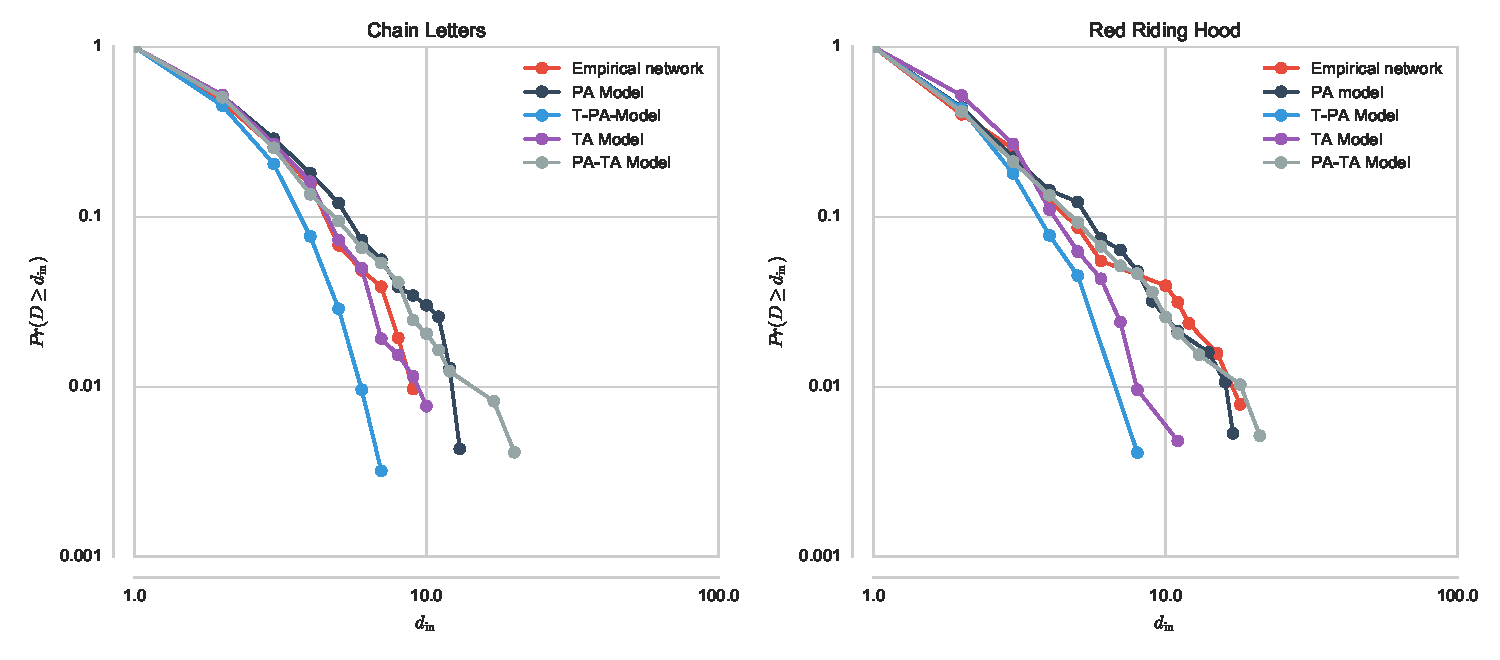
\includegraphics[width=\textwidth]{images/degree-comp.pdf}
\caption{Complementary cumulative in-degree distributions of the empirically derived network and simulations of the PA, T-PA, TA, and PA-TA modes. The left subplot shows the in-degree distribution of the chain letter network. The corresponding distributions of the four growing network models were obtained from a single simulation. The right subplot provides the same information for ``Red Riding Hood''.}
\label{fig:degree-model-comparisons}
\end{figure}

Figure \ref{fig:degree-model-comparisons} presents the complementary cumulative in-degree distributions of both story networks as well as those of the four proposed models. I will compare the in-degree distributions on the basis of their corresponding Gini coefficients $G$, which are presented in Table \ref{tab:gini-comparison}. The four growing network models are probabilistic and therefore results vary from simulation to simulation. The reported Gini coefficients are obtained by averaging 50 simulations. 

The PA model generates heavy-tailed in-degree distributions for ``Red Riding Hood'', of which the summarizing $G$ values are comparable to the empirical coefficient. The Gini coefficient of the chain letter network is much smaller than those produced by the PA model. As was expected, the time-span distributions of the PA model are negatively skewed (chain letters: median $\hat{\tau}= 0.7$; ``Red Riding Hood'': median $\hat{\tau}=0.5$) and the oldest nodes (i.e.\ the nodes that first enter the network) receive most of the incoming links over time. The three growing network models that take the age of nodes into account produce positively skewed time-span distributions in which younger nodes are preferred over older ones (chain letters: T-PA = 0.01, TA = 0.03, PA-TA = 0.04; ``Red Riding Hood'': T-PA = 0.06, TA = 0.07, PA-TA = 0.08). The Gini coefficients of the T-PA model are, however, rather small compared to the empirical coefficients. The temporal attractiveness (TA) model generates in-degree distributions that display the most similar degrees of inequality to those of the chain letter network. In the case of ``Red Riding Hood'', the best results are obtained by the PA-TA model.

\begin{table}
  \centering
  \begin{tabular}{lrrrrr}
  \toprule
                    & \multicolumn{5}{c}{Gini Coefficient}   \\ \midrule
                    & Empirical & PA   & T-PA & TA   & PA-TA \\ \cmidrule(r){2-6}
    Chain letters   & 0.36      & 0.41 & 0.29 & {\bf 0.36} & 0.41  \\
    Red Riding Hood & 0.43      & 0.41 & 0.29 & 0.37 & {\bf 0.43}  \\
  \bottomrule
  \end{tabular}
  \caption{Gini Coefficients of the two story networks (i.e.\ chain letters and ``Red Riding Hood'') and the four growing network models (i.e.\ PA, T-PA, TA, and PA-TA). The reported Gini coefficients are obtained by averaging 50 simulations for each of the four models of network growth. The empirical chain letter network displays an in-degree distribution which is most similar to those generated by the temporal attractiveness (TA) model. The in-degree distribution of the empirical ``Red Riding Hood'' network is most similar to the distributions generated by the Preferential Attachment Temporal Attractiveness (PA-TA) model.}
  \label{tab:gini-comparison}
\end{table}

\section{Discussion}\label{sec:networks-discussion}

In this chapter, I have studied the structure and evolution of story networks. Story networks, defined as non-hierarchical agglomerations of pre-textual relationships, represent streams of retellings in which retellers modify and adapt retellings in a gradual and accumulative way. The first challenge was to develop methods that allow us to automatically extract such story networks from raw text collections. To this end, I have proposed a clustering procedure, termed \emph{Bootstrap Neighbor Clustering}, which approaches the problem of pre-text selection as an open-set problem and attempts to bootstrap pre-textual story networks. I have constructed such story networks for two diachronic collections of retellings: a collection of paper chain letters and a collection of Dutch ``Red Riding Hood'' retellings. 

Using these extracted networks as a base, it was possible to provide a mechanistic understanding of story network growth and, by extension, of retellers' motivations for choosing particular story versions to base their retelling on. I hypothesized that stories are differentially preferred to function as a retelling's pre-text given three types of attractiveness: frequency-based, temporal, and model-based attractiveness. To gain more insight into the relations between stories and their pre-texts, I assessed the patterns of connectivity of the two story networks by performing a rigorous statistical analysis of their in-degree distributions. The in-degree distribution of ``Red Riding Hood'' displays heavy-tail properties that are well characterized by means of a power-law or log-normal model. Such heavy-tailness implies that a large proportion of stories have small in-degree values and only a few, yet significant number of stories function as pre-textual context for a large number of other stories. The heavy-tail distribution of ``Red Riding Hood'' contrasts with the relatively uniform in-degree distribution of the chain letter network, which was characterized as being exponential. 

In addition, I have demonstrated that retellings of chain letters and ``Red Riding Hood'' are published in relatively close temporal proximity. The effect of temporal attractiveness is most strongly observed in the chain letter corpus. Its story network displays a chain-like structure that is reminiscent of the letter's request to be redistributed within a short period of time. It was shown that the time-span distribution of the chain letters does not display a positive correlation with its corresponding in-degree distribution. Retellings of ``Red Riding Hood'', on the other hand, do exhibit a significant correlation between in-degree and age. These contrasting results can be linked to an important difference between the chain letter and ``Red Riding Hood'' retellings: Whereas retellers of ``Red Riding Hood'' can choose from a vast amount of story versions, chain letter retellers are requested to redistribute and retell one specific version. Moreover, it was shown that, in the retelling of chain letters, the mechanism of preferential attachment has no effect.

To explore which mechanisms potentially underlie the evolution of the two story networks, I have investigated a model of network growth. In addition to a preferential attachment mechanism, this model implements a form of model-based attractiveness which decays exponentially in time. The model that incorporates both preferential attachment and temporal attractiveness (PA-TA) best simulates the in-degree distribution of ``Red Riding Hood''. The more parsimonious temporal attractiveness (TA) model sufficed to account for the observed in-degree distribution of the chain letter network. This result concurs with the finding that the in-degree distribution of the chain letter network does not depend on age. Both models of network growth generate positively skewed time-span distributions that are comparable to the observed story network distributions. 

This being said, I wish to stress that there is not one true story network. In this chapter, I made a rather conservative and simplifying choice by investigating pre-textual relationships between stories on the basis of their vocabulary. However, the number of dimensions on which stories can be considered (dis)similar is virtually endless. In order to avoid falling into an `essentialist' trap, future research should first be directed toward studying different dimensions of story similarity (e.g.\ topics, motifs, genre) and their effect on the structure of story networks\autocite[Cf.][]{abello:2012}. A second point of future research is to further explore macroscopic properties of story networks. While the present study mainly focused on the in-degree distributions of story networks, one needs to investigate other general principles governing their structure and evolution in order to obtain a more profound understanding of story networks. Many complex real-world networks can be characterized as so-called `small-world networks', which exhibit two fundamental properties: (i) locally connected groups of nodes and (ii) a short average shortest path length between nodes~\autocite{watts:1998,newman:2003}. I take it to be an interesting question whether story networks display this small-world property. In this scenario, stories would be connected to only a few other stories, while at the same time all stories in the network would be connected to each other through only a few intermediate steps. Another principle governing many real-world networks is a modular structure. Networks with modular structure are hierarchically organized into local groups of densely connected nodes, with a low density of connections \emph{between} groups\autocite{newman:2003}. A modularity analysis of story networks could reveal that stories with high in-degrees function as bridges between local `story communities' and integrate them into a single network\autocite{carron:2012}.